\documentclass[conference]{IEEEtran}
\IEEEoverridecommandlockouts

\usepackage{amsmath,amssymb}
\usepackage{graphicx}
\usepackage{xcolor}
\usepackage{hyperref}
\usepackage{booktabs}
\usepackage{tabularx}
\usepackage{array}
\usepackage{url}
\usepackage{tikz}
\usetikzlibrary{arrows.meta,positioning,fit,calc}

\newcolumntype{Y}{>{\raggedright\arraybackslash}X}

\hypersetup{
    colorlinks=true,
    linkcolor=blue,
    filecolor=magenta,
    urlcolor=cyan,
    citecolor=blue,
    pdfborder={0 0 0}
}

\begin{document}

\title{Caduceus-Flux: Mikroservis Tabanli Ag Emulasyon Platformu icin Butunlesik Mimari, Servis Detaylari ve Deneysel Altyapi}

\author{\IEEEauthorblockN{Yazarlar}
\IEEEauthorblockA{\textit{Bolum} \\
\textit{Universite}\\
Sehir, Ulke \\
email@universite.edu}}

\maketitle

\begin{abstract}
Bu calisma, Caduceus-Flux adli mikroservis tabanli ag emulasyon platformunun mimarisini, servislerini ve calisma modelini ayrintili bir konferans yayini olarak sunar. Platform, Mininet/Containernet/Mininet-WiFi tabanli emulasyon cekirdegini es zamanli coklu topoloji calistirma, topoloji basina izole altyapi, snapshot/restore, programlanabilir veri duzlemi (P4), gozlemlenebilirlik ve AI/LLM destekli kontrol ile butunlestirir. Bu sayede deney tekrar edilebilirligi, otomasyon ve niyet tabanli yonetim hedefleri icin entegre bir arastirma ortami ortaya cikar. Makale; katmanli mimariyi, mikroservislerin sorumluluk ayrimini, veri ve mesaj katmanini, UI akislari ve proxy tabanli dis arayuz erisimlerini, snapshot/restore zincirini ve LLM-MANO karar dongulerini sistematik bicimde ele alir. Ayrica servis bazli isleyis, veri modeli baglantilari ve degerlendirme planini matrislerle sunar.
\end{abstract}

\begin{IEEEkeywords}
ag emulasyonu, mikroservis mimarisi, topoloji izolasyonu, gozlemlenebilirlik, AI/LLM kontrolu, NFV MANO, P4
\end{IEEEkeywords}

\section{Giris}
Ag emulasyon platformlari SDN, routing protokolleri, kablosuz senaryolar ve NFV deneyleri icin temel altyapiyi saglar. Ancak klasik monolitik yaklasimlar, runtime degisiklikleri icin yeniden baslatma gereksinimi, zayif coklu-topoloji izolasyonu, sinirli telemetri ve otomasyon eksikligi gibi engeller barindirir. Caduceus-Flux, bu sinirlari mikroservis tabanli bir kontrol duzlemi, topolojiye ozel izolasyon mekanizmalari ve veri akisi odakli gozlemlenebilirlik yiginlari ile asmayi hedefler.

\section{Motivasyon ve Problem Tanim}
Literaturdeki araclar belirli fonksiyonlari saglasa da, tum F1--F10 fonksiyon setini ayni platformda birlestirme konusunda belirgin eksikler bulunur. Topoloji ciziminden calistirmaya, runtime degisimden P4 entegrasyonuna, veritabani kaliciligindan otomatik topoloji uretimine kadar uzanan genis kapsamli bir deney altyapisi, bugune kadar birden fazla arac ve el ile entegrasyon gerektirmistir. Caduceus-Flux, bu butunlesik ihtiyaci tek bir platformda karsilamayi hedefler; ayni zamanda LLM-MANO karar dongulerinin deneysel dogrulamasina imkan veren AI/LLM kontrol katmanini sisteme dahil eder.

\section{Ilgili Calismalar}
Mininet~\cite{mininet}, Containernet~\cite{containernet} ve Mininet-WiFi~\cite{mininet-wifi} hizli prototipleme icin guclu bir temel sunar; ancak monolitik mimari ve sinirli otomasyon nedeniyle kapsamli arastirma deneyleri icin yetersiz kalir. SDN denetleyicileri (ONOS~\cite{onos}, OpenDaylight~\cite{odl}) ve P4 ekosistemi, veri duzleminde yuksek esneklik saglasa da bu bilesenlerin deneysel platformlara entegrasyonu genellikle ad-hoc yontemlerle yapilir. Caduceus-Flux, bu bilesenleri bir mikroservis mimarisi altinda dogrudan entegre ederek hem kontrol hem veri duzlemini tek bir deneysel ortamda birlestirir.

\section{Sistem Mimarisi}
Caduceus-Flux mimarisi, katmanli bir yaklasimla tasarlanmistir ve her katmanin sorumlulugu acik sekilde ayrilmistir. Arayuz katmani (Web UI ve API istemcileri) Nginx ve MCP Server uzerinden sisteme erisir. MCP Server servis kesfi ve path-bazli routing yapar. Kontrol duzlemi; topoloji, orkestrasyon, protokol/cihaz yonetimi, snapshot/restore, P4, monitoring, AI/LLM kontrolu ve MANO/NFV servislerini icerir. Emulasyon runtime katmani, her topoloji icin ayrilan container icinde Mininet/Containernet/Mininet-WiFi cekirdegi calistirir ve gRPC ile kontrol edilir. Paylasimli altyapi katmani Postgres, MongoDB, Redis, InfluxDB, Prometheus, Kafka, RabbitMQ ve Consul gibi servisleri barindirir. Izolasyon modu etkinse, topolojiye ozel altyapi setleri (InfluxDB, Grafana, Consul, RabbitMQ, Kafka, Portainer vb.) dinamik olarak uretilir.

\begin{figure}[htbp]
\centering
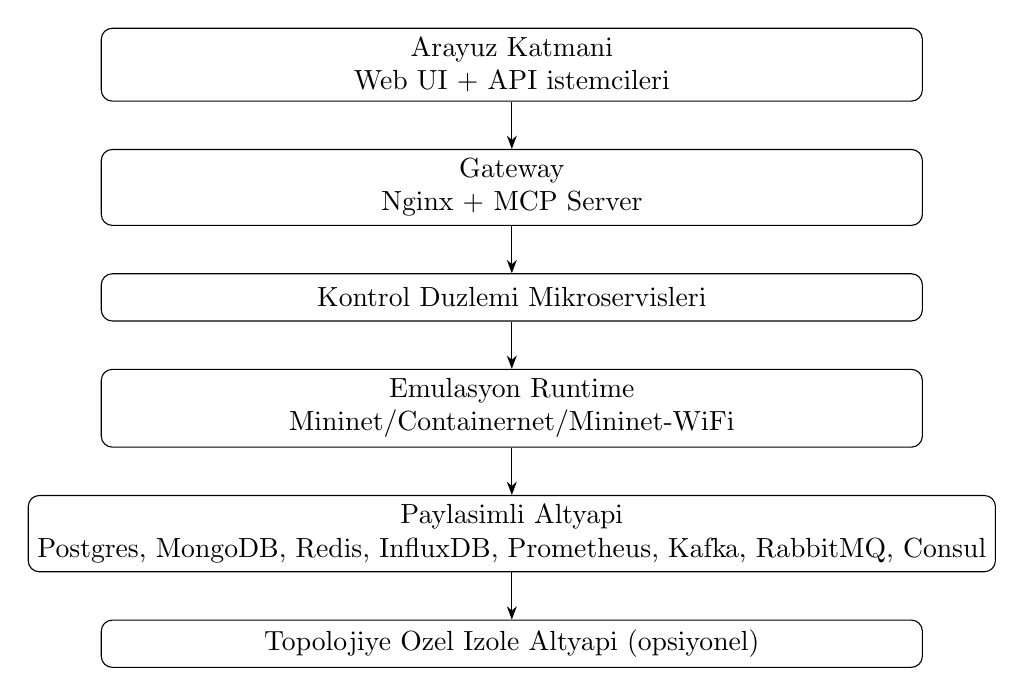
\begin{tikzpicture}[
  node distance=6mm,
  box/.style={draw, rounded corners, align=center, minimum width=0.86\linewidth, minimum height=6mm}
]
\node[box] (ui) {Arayuz Katmani\\Web UI + API istemcileri};
\node[box, below=of ui] (gw) {Gateway\\Nginx + MCP Server};
\node[box, below=of gw] (cp) {Kontrol Duzlemi Mikroservisleri};
\node[box, below=of cp] (rt) {Emulasyon Runtime\\Mininet/Containernet/Mininet-WiFi};
\node[box, below=of rt] (shared) {Paylasimli Altyapi\\Postgres, MongoDB, Redis, InfluxDB, Prometheus, Kafka, RabbitMQ, Consul};
\node[box, below=of shared] (iso) {Topolojiye Ozel Izole Altyapi (opsiyonel)};
\draw[-{Stealth}] (ui) -- (gw);
\draw[-{Stealth}] (gw) -- (cp);
\draw[-{Stealth}] (cp) -- (rt);
\draw[-{Stealth}] (rt) -- (shared);
\draw[-{Stealth}] (shared) -- (iso);
\end{tikzpicture}
\caption{Caduceus-Flux katmanli mimari gorunumu.}
\label{fig:arch}
\end{figure}

\section{Servisler (Tek Tek Detayli)}
Bu bolumde 21 mikroservis tek tek aciklanir. Her servisin rolu, veri durumu, tipik akislari ve entegrasyonu ozetlenir.

\subsection{Topology Service (8001)}
Topology Service proje/topoloji verisinin kaynagini olusturur. Projeler, topolojiler, node/link bilgileri ve controller tanimlari Postgres uzerinde kalici tutulur. UI tarafinda /projects ve /topology/:id ekranlari bu servise dogrudan baglidir. Import/export ve P4 taslaklari gibi fonksiyonlar icin diger servislerle (Export/Import, P4 Manager) birlikte calisir.

\subsection{Orchestrator Service (8002)}
Orchestrator emulasyon yasam dongusunu yonetir: emulasyon baslatma/durdurma, gRPC port tahsisi, altyapi ensure ve izole altyapi stack uretimi. Runtime state Redis hash yapilarinda tutulur (active emulations ve algorithm runs). UI tarafinda network-manager, topology editor, snapshots ve infrastructure ekranlari bu servis uzerinden isletilir.

\subsection{Protocol Manager (8003)}
Protokol plugin tabanli yonetim saglar. Configure/enable/disable/hot-swap akislari ile OSPF, BGP, ISIS, RIP ve static protokollerin runtime gecisleri desteklenir. Stateless calisir; konfig dogrulama ve gecislerde runtime ile etkileşir. Genellikle MCP/AI ya da API istemcilerince cagirilir.

\subsection{Device Manager (8004)}
Calisan emulasyona runtime cihaz ekleme/silme/guncelleme yapar. Runtime cihazlar Postgres runtime
table’da izlenir. UI tarafinda network-manager ve monitoring ekranlari cihaz listesi ve operasyonlari icin bu servise baglanir.

\subsection{Controller Manager (8005)}
SDN controller lifecycle’ini yonetir (osken, ryu, odl, onos, custom). Container lifecycle, log ve status saglanir. Proxy mekanizmalari ile controller UI’lari network-manager ve infrastructure uzerinden acilabilir.

\subsection{Snapshot Service (8006)}
Snapshot Service snapshot/restore akisini ve schedule mekanizmasini yonetir. Snapshot metadata Postgres’te, state verileri MongoDB’de saklanir. UI tarafinda /snapshots ve /schedules ekranlari bu servis uzerinden calisir. CRIU ve Docker commit tabanli checkpoint mekanizmalari desteklenir.

\subsection{WebShell Service (8007)}
WebSocket uzerinden Mininet CLI ve cihaz namespace komutlari sunar. Oturumlar in-memory tutulur ve emulation state json dosyasindan baglam okunur. Topology editor ve network-manager uzerindeki WebShell/MininetCLI modallari ile entegredir.

\subsection{Export/Import Service (8008)}
Topoloji verisini Mininet/Mininet-WiFi/Containernet betikleri, GraphML, JSON ve YAML formatlarinda disari verir. UI tarafinda proje import ve network-manager export islevleri bu servisi kullanir.

\subsection{Topology Generator (8009)}
Tree, mesh, ring, star ve fat-tree gibi algoritmalarla otomatik topoloji uretir. Genellikle API/MCP uzerinden tetiklenir ve Topology Service’e uygulanir.

\subsection{P4 Manager (8010)}
P4 programlarini derler, artefact dosyalarini saklar ve BMv2 switchlerle entegre eder. P4 programlari dosya/volume uzerinden yonetilir. UI’da Topology Editor P4 paneli ve Device Properties uzerinden erisim saglanir.

\subsection{Monitoring Service (8011)}
Emulasyon runtime’dan gRPC ile metrik toplar ve InfluxDB/Prometheus’a yazar. Interface ve device metrikleri, switch flow bilgileri ve routing tablolarina erisim saglar. Monitoring ve network-manager ekranlari bu servis uzerinden calisir.

\subsection{MCP Server (8012)}
Tum mikroservisleri tek bir API altinda toplar, servis kesfi ve OpenAPI proxy yapar. UI tarafinda butun /api cagirilari MCP uzerinden gecer. Dokumantasyon /docs uzerinden sunulur.

\subsection{Metrics Collector (8013)}
Runtime metriklerini gRPC stream uzerinden alir ve Kafka’ya aktarir. Buffer ve batch mekanizmalari ile throughput kontrolu saglar. Test paneli uzerinden start/stop edilebilir.

\subsection{AI Gateway (8014)}
LLM saglayicilarini tek API uzerinde birlestirir (OpenAI, Anthropic, Gemini, Ollama). MCP uzerinden API cagri uretimi ve execution saglar. AI agent, thread ve tool-call kayitlari Postgres uzerinde tutulur. UI’da /ai-console ve /ai-settings ekranlari bu servisle calisir.

\subsection{MANO Service (8015 + 50052)}
VNFD/NSD katalogu ve VNF/NS lifecycle operasyonlarini yerel olarak yonetir. Postgres uzerinde mano_vnfd, mano_nsd, mano_ns_instance, mano_vnf_instance ve mano_operation tablolari kullanilir. Network-manager uzerindeki MANO tab’i bu servisle entegredir.

\subsection{Config Service (8016)}
JSON tabanli control-config akisini validate/apply eder. MCP uzerinden Orchestrator ve diger servislere istek zinciri kurar. UI’da control-config paneli (network-manager) bu servisi kullanir.

\subsection{Decision Engine (8017)}
Kafka’dan islenmis metrikleri alir ve anomali, attack, routing ve MANO kararlarini paralel uretir. State in-memory tutulur. Monitoring ve AI katmanina karar sinyali saglar.

\subsection{MCP Tool Hub (8018)}
Dis MCP server kayitlari ve policy (read-only, allowlist) yonetimi saglar. Consul KV uzerinden kayit tutar. AI Gateway bu registry’yi kullanarak guvenli proxy uygular.

\subsection{OSM Connector (8020)}
ETSI OSM NBI’yi proxy eder, token cache tutar ve OSM kaynaklarini UI’da gorunur hale getirir. OSM UI, infra-proxy endpointleri uzerinden acilir.

\subsection{VIM Emulator (6001)}
OpenStack benzeri Keystone/Nova/Neutron API saglar. MemoryStore uzerinde image, network, server ve port state’i tutar. OSM tarafindan VIM olarak kullanilir.

\subsection{MCP Proxy (8000)}
Generic HTTP proxy olarak calisir. Read-only ve path filtreleme politikasi uygular. Dis servislerin guvenli okunmasinda kullanilir.

\subsection{Emulation Container (gRPC Runtime)}
Mininet/Containernet/Mininet-WiFi runtime’ini tek container icinde calistirir. gRPC API ile device/link islemleri, komut calistirma, metrik streaming ve snapshot bileşenlerini saglar. Orchestrator ve diger servisler bu runtime ile dogrudan etkilesir.

\section{Matrisler}
\subsection{Detayli Mikroservis Matrisi}
\begin{table*}[t]
\caption{Mikroservis Detay Matrisi (Port, Container, Bagimlilik, Mesaj Akisi)}
\label{tab:svc_matrix}
\centering
\scriptsize
\setlength{\tabcolsep}{3pt}
\begin{tabularx}{\textwidth}{l c l Y Y}
\toprule
Servis & Port & Container & Bagimliliklar (Ozet) & Mesaj/Topic (Ozet) \\
\midrule
Topology Service & 8001 & caduceus-topology-service & Postgres, RabbitMQ, Consul & RabbitMQ: topology.* \\
Orchestrator & 8002 & caduceus-orchestrator-service & Docker, Redis, RabbitMQ, Consul & RabbitMQ: emulation.* \\
Protocol Manager & 8003 & caduceus-protocol-manager-service & Consul, RabbitMQ & RabbitMQ: protocol.* \\
Device Manager & 8004 & caduceus-device-manager-service & Postgres, RabbitMQ, Orchestrator & RabbitMQ: device.* \\
Controller Manager & 8005 & caduceus-controller-manager-service & Docker, RabbitMQ, Consul & (event bus) \\
Snapshot Service & 8006 & caduceus-snapshot-service & Postgres, MongoDB, Docker, RabbitMQ & (event bus) \\
WebShell Service & 8007 & caduceus-webshell-service & Redis, Docker, gRPC Runtime & (yok) \\
Export/Import Service & 8008 & caduceus-export-import-service & Topology DB, Consul & (yok) \\
Topology Generator & 8009 & caduceus-topology-generator-service & Consul & (yok) \\
P4 Manager & 8010 & caduceus-p4-manager-service & Docker, Consul & (yok) \\
Monitoring Service & 8011 & caduceus-monitoring-service & InfluxDB, Prometheus, Kafka & Kafka: metrics.raw/metrics.processed \\
MCP Server & 8012 & caduceus-mcp-server & Consul, RabbitMQ & (gateway) \\
Metrics Collector & 8013 & caduceus-metrics-collector-service & Kafka, gRPC Runtime & Kafka: metrics.raw \\
AI Gateway & 8014 & caduceus-ai-gateway-service & Postgres, MCP Server & (MCP calls) \\
MANO Service & 8015/50052 & caduceus-mano-service & Postgres, Orchestrator & Kafka: mano.events (opsiyonel) \\
Config Service & 8016 & caduceus-config-service & MCP Server & (yok) \\
Decision Engine & 8017 & caduceus-decision-engine-service & Kafka & Kafka: metrics.processed, alerts.* \\
MCP Tool Hub & 8018 & caduceus-mcp-tool-hub-service & Consul & (registry) \\
OSM Connector & 8020 & caduceus-osm-connector-service & OSM NBI, Consul & (proxy) \\
VIM Emulator & 6001 & caduceus-vimemu-service & Orchestrator, Runtime & (proxy) \\
MCP Proxy & 8000 & mcp-\{service\} & Upstream HTTP & (proxy) \\
Emulation Runtime & 50051 & caduceus-emu-\{topology\} & Mininet/Containernet/Mininet-WiFi & gRPC streams \\
\bottomrule
\end{tabularx}
\end{table*}

\subsection{Veri Katmani Matrisi}
\begin{table}[htbp]
\caption{Veri Katmani Kullanimi (Ozet)}
\label{tab:data_matrix}
\centering
\scriptsize
\begin{tabularx}{\linewidth}{l Y}
\toprule
Bilesen & Veri Katmani \\
\midrule
Topology Service & PostgreSQL (projects, topologies, nodes, links, controllers, network_configurations) \\
Orchestrator & Redis (active emulations, algorithm runs) \\
Snapshot Service & PostgreSQL (metadata) + MongoDB (state, blobs) \\
Monitoring & InfluxDB + Prometheus \\
AI Gateway & PostgreSQL (ai\_provider\_config, ai\_agent, ai\_thread, ai\_message, ai\_tool\_call, ai\_run, ml\_model) \\
MANO Service & PostgreSQL (mano\_vnfd, mano\_nsd, mano\_ns\_instance, mano\_vnf\_instance, mano\_operation) \\
Decision Engine & In-memory + Kafka streams \\
\bottomrule
\end{tabularx}
\end{table}

\subsection{Mesajlasma/Topic Matrisi}
\begin{table}[htbp]
\caption{Mesajlasma Katmani ve Topic/Exchange Ozetleri}
\label{tab:msg_matrix}
\centering
\scriptsize
\begin{tabularx}{\linewidth}{l Y}
\toprule
Katman & Topic/Exchange Ozetleri \\
\midrule
RabbitMQ & topology.* (topoloji olaylari), device.* (runtime cihaz olaylari), protocol.* (protokol degisimleri), emulation.* (emulasyon lifecycle) \\
Kafka & metrics.raw (ham metrik akisi), metrics.processed (islenmis metrik akisi), alerts.* (anomaly/decision uyarilari) \\
\bottomrule
\end{tabularx}
\end{table}

\subsection{UI-Servis Haritasi}
\begin{table*}[t]
\caption{UI Ekranlari ve Servis Baglantilari}
\label{tab:ui_matrix}
\centering
\scriptsize
\begin{tabularx}{\textwidth}{l Y}
\toprule
UI Ekrani & Servisler \\
\midrule
/projects & Topology Service, Export/Import \\
/topology/:id & Topology Service, Orchestrator, WebShell, P4 Manager \\
/network-manager & Orchestrator, Device Manager, Controller Manager, Monitoring, AI Gateway, MANO, Config Service \\
/monitoring/:id & Monitoring Service, Device Manager \\
/snapshots & Snapshot Service, Orchestrator \\
/schedules & Snapshot Service \\
/ai-console & AI Gateway, MCP Tool Hub \\
/ai-settings & AI Gateway \\
/ml-models & AI Gateway (ML registry) \\
/infrastructure & Orchestrator (infra status/ensure) + proxy UI \\
\bottomrule
\end{tabularx}
\end{table*}

\section{Diagramlar}
\subsection{Deployment Diyagrami}
\begin{figure}[htbp]
\centering
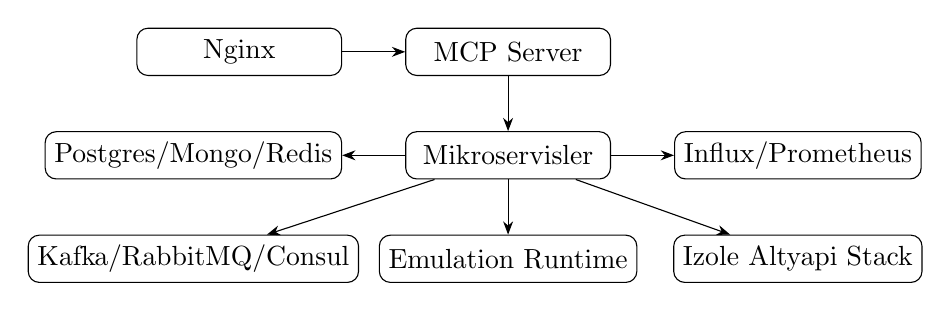
\begin{tikzpicture}[
  node distance=7mm and 8mm,
  box/.style={draw, rounded corners, align=center, minimum width=26mm, minimum height=6mm},
  group/.style={draw, dashed, rounded corners, inner sep=4mm}
]
\node[box] (ng) {Nginx};
\node[box, right=of ng] (mcp) {MCP Server};
\node[box, below=of mcp] (svc) {Mikroservisler};
\node[box, below=of svc] (rt) {Emulation Runtime};
\node[box, left=of svc] (db) {Postgres/Mongo/Redis};
\node[box, right=of svc] (obs) {Influx/Prometheus};
\node[box, below=of db] (mq) {Kafka/RabbitMQ/Consul};
\node[box, below=of obs] (iso) {Izole Altyapi Stack};
\draw[-{Stealth}] (ng) -- (mcp);
\draw[-{Stealth}] (mcp) -- (svc);
\draw[-{Stealth}] (svc) -- (rt);
\draw[-{Stealth}] (svc) -- (db);
\draw[-{Stealth}] (svc) -- (obs);
\draw[-{Stealth}] (svc) -- (mq);
\draw[-{Stealth}] (svc) -- (iso);
\end{tikzpicture}
\caption{Deployment gorunumu (tikz).}
\label{fig:deploy}
\end{figure}

\subsection{LLM-MCP Kontrol Akisi}
\begin{figure}[htbp]
\centering
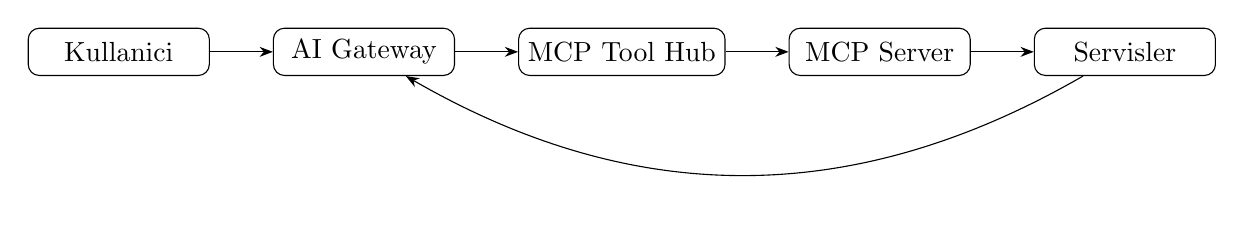
\begin{tikzpicture}[
  node distance=8mm,
  box/.style={draw, rounded corners, align=center, minimum width=23mm, minimum height=6mm}
]
\node[box] (u) {Kullanici};
\node[box, right=of u] (ai) {AI Gateway};
\node[box, right=of ai] (hub) {MCP Tool Hub};
\node[box, right=of hub] (mcp) {MCP Server};
\node[box, right=of mcp] (svc) {Servisler};
\draw[-{Stealth}] (u) -- (ai);
\draw[-{Stealth}] (ai) -- (hub);
\draw[-{Stealth}] (hub) -- (mcp);
\draw[-{Stealth}] (mcp) -- (svc);
\draw[-{Stealth}] (svc) to[bend left] (ai);
\end{tikzpicture}
\caption{LLM tabanli MCP kontrol akisi.}
\label{fig:seq_llm}
\end{figure}

\subsection{Snapshot/Restore Akisi}
\begin{figure}[htbp]
\centering
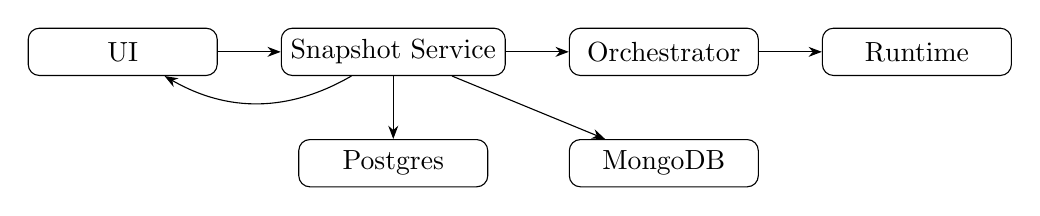
\begin{tikzpicture}[
  node distance=8mm,
  box/.style={draw, rounded corners, align=center, minimum width=24mm, minimum height=6mm}
]
\node[box] (ui) {UI};
\node[box, right=of ui] (ss) {Snapshot Service};
\node[box, right=of ss] (orch) {Orchestrator};
\node[box, right=of orch] (rt) {Runtime};
\node[box, below=of ss] (pg) {Postgres};
\node[box, below=of orch] (mg) {MongoDB};
\draw[-{Stealth}] (ui) -- (ss);
\draw[-{Stealth}] (ss) -- (orch);
\draw[-{Stealth}] (orch) -- (rt);
\draw[-{Stealth}] (ss) -- (pg);
\draw[-{Stealth}] (ss) -- (mg);
\draw[-{Stealth}] (ss) to[bend left] (ui);
\end{tikzpicture}
\caption{Snapshot/restore islem akisi.}
\label{fig:seq_snapshot}
\end{figure}

\subsection{Telemetri Pipeline}
\begin{figure}[htbp]
\centering
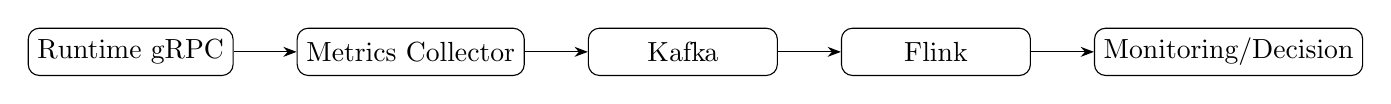
\begin{tikzpicture}[
  node distance=8mm,
  box/.style={draw, rounded corners, align=center, minimum width=24mm, minimum height=6mm}
]
\node[box] (rt) {Runtime gRPC};
\node[box, right=of rt] (mc) {Metrics Collector};
\node[box, right=of mc] (k) {Kafka};
\node[box, right=of k] (f) {Flink};
\node[box, right=of f] (md) {Monitoring/Decision};
\draw[-{Stealth}] (rt) -- (mc);
\draw[-{Stealth}] (mc) -- (k);
\draw[-{Stealth}] (k) -- (f);
\draw[-{Stealth}] (f) -- (md);
\end{tikzpicture}
\caption{Telemetri pipeline akisi.}
\label{fig:seq_metrics}
\end{figure}

\section{Degerlendirme Plani}
Degerlendirme, kontrol-duzlemi performansini ve streaming pipeline verimliligini olcmeyi hedefler. Emulasyon baslatma gecikmesi, runtime cihaz ekleme suresi, protokol hot-swap gecis suresi ve snapshot capture/restore gecikmesi temel metriklerdir. Coklu topoloji senaryolarinda kaynak tuketimi ve throughput analiz edilir. Gozlemlenebilirlik katmaninin ek yuku Kafka throughput ve Flink latency gibi parametrelerle incelenir. MANO ve AI destekli senaryolarda operasyonel dogruluk ve stabilite olculur.

\section{Sonuc}
Caduceus-Flux, mikroservis tabanli mimariyi Mininet/Containernet/Mininet-WiFi cekirdegi ile butunlestiren; izolasyon, gozlemlenebilirlik, otomasyon ve tekrarlanabilirlik eksenlerinde kapsamli bir arastirma platformu sunar. Bu calisma, platformun mimari prensiplerini, servis bazli isleyisini, veri katmanini ve LLM-MANO entegrasyonunu akademik bir cati altinda toplamis; sistemin yeniliklerini detayli bir sekilde ortaya koymustur.

\begin{thebibliography}{99}

\bibitem{mininet}
B. Lantz, B. Heller, and N. McKeown, ``A network in a laptop: rapid prototyping for software-defined networks,'' in \textit{Proc. 9th ACM Workshop on Hot Topics in Networks (HotNets)}, 2010.

\bibitem{containernet}
M. Peuster, H. Karl, and S. van Rossem, ``MeDICINE: Rapid prototyping of production-ready network services in multi-PoP environments,'' in \textit{Proc. IEEE Conference on Network Function Virtualization and Software Defined Networks (NFV-SDN)}, 2016.

\bibitem{mininet-wifi}
R. R. Fontes, S. Afzal, S. H. B. Brito, M. A. S. Santos, and C. E. Rothenberg, ``Mininet-WiFi: Emulating software-defined wireless networks,'' in \textit{Proc. 11th International Conference on Network and Service Management (CNSM)}, 2015.

\bibitem{ns3}
``ns-3: A discrete-event network simulator,'' https://www.nsnam.org/

\bibitem{onos}
P. Berde et al., ``ONOS: Towards an open, distributed SDN OS,'' in \textit{Proc. 3rd ACM Workshop on Hot Topics in Software Defined Networking (HotSDN)}, 2014.

\bibitem{odl}
``OpenDaylight: Open source SDN platform,'' https://www.opendaylight.org/

\end{thebibliography}

\end{document}
